\subsection{Ablations and controlled negative controls}
\label{sec:pricing}

The surcharge is off by default ($\theta=0$), and yield-record-guided local search runs with the same setting in all four configurations, so neither affects the comparisons between them.

On the $\MatrixCells$-instance batch of Section~\ref{sec:whichcongestion}, valid here because the cost of these operators, unlike that of dispatching, does not depend on pruning, turning off yield-record feedback gives a relative gain of \GainCertMatrix{} (significant on $1$ instance) and turning off staggering gives \GainStaggerMatrix{} (significant on $2$). Neither is positive: under an equal wall-clock budget, these decodes are better spent on population evolution. The local search consumes a large share of all decodes, yet fewer than one in fifty of its neighbours improve makespan although the neighbourhood is small and well targeted (Section~\ref{sec:ls}), and three refinements of its operators were each not significant under an equal number of evaluations, so the signal itself fails.

The surcharge counts again a delay that fitness already includes (Section~\ref{sec:interface}), so it adds no information, but its cost must be measured. On two instances outside Families A/B/C (Table~\ref{tab:batches}), with the path-planning search width fixed, every surcharge coefficient $\theta$ tried worsens makespan significantly at equal wall-clock time, flat over a ten-fold range, whereas at an equal number of evaluations the difference cannot be distinguished from zero. Routing with a surcharge completes only about one fifth as many evaluations, because a second criterion removes total-order dominance (Lemma~\ref{lem:label}) and requires a multi-label search whose overhead is the same at every $\theta$. Nor is $\theta$ a useful tuning parameter: the cumulative surcharge is too small to reorder arrivals, so makespan is unchanged over two orders of magnitude until the surcharge outweighs the arrival time and the double counting worsens it sharply. An interface that passes a quantity already contained in the objective of the receiving layer is therefore harmful under our protocol.

\paragraph{Dilution and overhead.}
\label{sec:whycost}
A yield record names what is needed to remove one corridor delay, but makespan is set by a chain: once that delay is removed, another constraint usually becomes tight, so makespan improves by far less than the yielding time removed. The same dilution leaves reservation-table-aware dispatching only a few percentage points, lost in noise at a cost multiple of \CostMultBefore{} and significant in the pooled data once Section~\ref{sec:speedup} lowered it to \CostMultAfter{}. Local search thus fails because too little reduction survives dilution, whereas dispatching initially failed because each evaluation cost too much; dispatching is therefore a mechanism contribution, and yield-record-guided local search only a controlled negative control.


\subsection{The cost law and the effect of the two speed-ups}
\label{sec:costlaw}

Under a fixed wall-clock budget, the cost per evaluation and the number of evaluations trade off against each other (Figure~\ref{fig:protocol}): the cost spans about two orders of magnitude, and the open loop completes the most evaluations in about one fifth of the wall-clock time. An equal number of generations lets a costlier configuration use more compute and asks whether extra routing improves the ranking within a generation; equal wall-clock time asks whether makespan falls within the same time. The two conventions disagree: before the speed-ups, reservation-table-aware dispatching is \GainProbeSameGen{} ($p\PProbeSameGen$) at equal generations but only \GainProbeSameClock{} ($p\PProbeSameClock$) at equal wall-clock time, so we report both.

\begin{figure}[t]
\centering
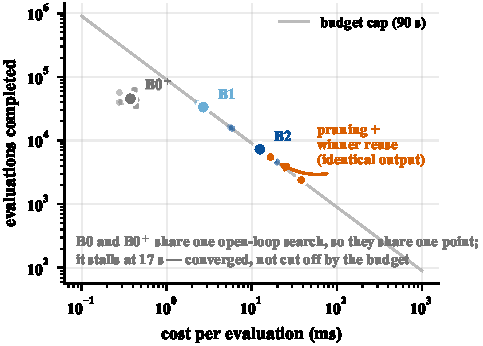
\includegraphics[width=\columnwidth]{fig/fig_protocol.pdf}
\Description{A log-log scatter of cost per evaluation against evaluations
completed, with a grey hyperbola for the 90-second budget cap and orange
markers for the pruning ablation.}
\caption{Cost per evaluation against evaluations completed under the shared $90$-second cap (grey hyperbola).
The closed-loop configurations use the full budget; the open loop (B0 and B0$^+$ share one point) is ended by early stopping after about $17$\,s.
Pale points: three instances; filled points: their geometric mean. Orange: pruning and winner-path reuse off and on.}
\label{fig:protocol}
%% From fig/fig_protocol.py; ladder_cost.csv and prune_ablation.csv.
%% fig:protocols (two-convention comparison) dropped; the pair
%% \GainProbeSameGen / \GainProbeSameClock is reported in the text.
\end{figure}

The cost law follows from the trial query: it raises the routing calls per transport task from $2$ to at most $2N_A$, so cost grows linearly with fleet size, while pruning cuts fewer calls as fleet and contention grow (\RouteCallCutHi{} on the least congested self-check instance, \RouteCallCutLo{} on the largest fleet). The law predicts a fleet size beyond which the trial-query cost offsets the gain; across the four vehicle-to-arm levels of Section~\ref{sec:whichcongestion} the sign alternates and no instance is significant, so the law is measured but this bound is not confirmed.

Because the dispatching rule and the speed-ups were introduced one after the other, a separate control changes only pruning and winner-path reuse, with the same instances, seeds and budget. They change neither the selected vehicle nor the timetable (Proposition~\ref{prop:speedup_equiv}): for six random chromosomes on each of six instances, makespans and dispatch sequences are identical bit for bit in all $36$ cases while routing calls fall by \RouteCallCut{}, so any difference comes only from the compute saved. Switching them on lowers makespan by a further \GainPrune{} ($p\PPrune$; Table~\ref{tab:prune}). The same rule thus moves from \GainProbePre{} before the speed-ups ($0$ of the $\MatrixCells$ instances significant) to significantly positive after them, without any change of selection.

\begin{table}[t]
\caption{Pruning and winner-path reuse off versus on (bold: adopted setting). Same instances, seeds and wall-clock time; $n=60$ pairs, two-sided Wilcoxon signed-rank test ($^{***}p<0.001$). Ratios take the off value as denominator.}
\label{tab:prune}
\small
%% Regenerated from prune_ablation.csv by gen_tables_ladder.py.
%% 由 tab/gen_tables_ladder.py 生成,请勿手工编辑
%% 数据源:clbs/output/baseline_ladder.csv 等,见脚本首部
\begin{tabular}{@{}lrrrrrr@{}}
\toprule
& & \multicolumn{2}{c}{$C_{\max}$ (time units)} & & Eval.\ count ratio & Speedup per eval. \\
\cmidrule(lr){3-4}
Instance & Contention & Off & \textbf{On} & $\Delta C_{\max}$ & (on/off) & (off/on) \\
\midrule
A funnel & 31.9\% & 44.80 & 42.10 & $-6.03\%$ & 2.21$\times$ & 2.23$\times$ \\
A high & 30.9\% & 41.60 & 37.70 & $-9.37\%$ & 2.40$\times$ & 2.41$\times$ \\
A low & 11.8\% & 60.50 & 57.00 & $-5.79\%$ & 2.79$\times$ & 2.81$\times$ \\
B NA/NM 0.5 & 15.8\% & 66.70 & 65.10 & $-2.40\%$ & 2.11$\times$ & 2.11$\times$ \\
B NA/NM 1.0 & 30.2\% & 51.90 & 48.90 & $-5.78\%$ & 2.31$\times$ & 2.31$\times$ \\
B NA/NM 2.0 & 32.4\% & 44.50 & 42.20 & $-5.17\%$ & 1.98$\times$ & 2.01$\times$ \\
\midrule
\emph{Pooled} (60 pairs) & --- & --- & --- & $-5.60\%^{***}$ & \multicolumn{2}{r}{50/0/10,\ $<10^{-4}$} \\
\midrule
\multicolumn{7}{@{}l@{}}{\footnotesize HL pseudomedian and $95\%$ CI:$-4.72$ $[-6.34,-3.55]$\,\%} \\
\bottomrule
\end{tabular}

\end{table}

\subsection{Case study: Gantt chart and critical chain on the funnel instance}
\label{sec:casestudy}

Aggregate numbers do not show what happens inside one solve, so Figure~\ref{fig:case} places B0 and B2 side by side on one funnel instance.
In the open-loop solution, yielding waits cluster on the corridors near the load/unload point $v_0$ and on a few vehicles. The closed-loop solution greatly reduces them and assigns several operations to an arm that is not the fastest (Eq.~\eqref{eq:reassign}), trading a longer processing time for a less congested path; its more even vehicle load follows from these two effects rather than from a separate mechanism.
Labelled as in Table~\ref{tab:attrib}, the B0 critical chain contains a substantial share of \texttt{corridor} links; on B2 they largely give way to \texttt{machine} and \texttt{upstream} links, the dilution of Section~\ref{sec:whycost}.

\begin{figure*}[t]
\centering
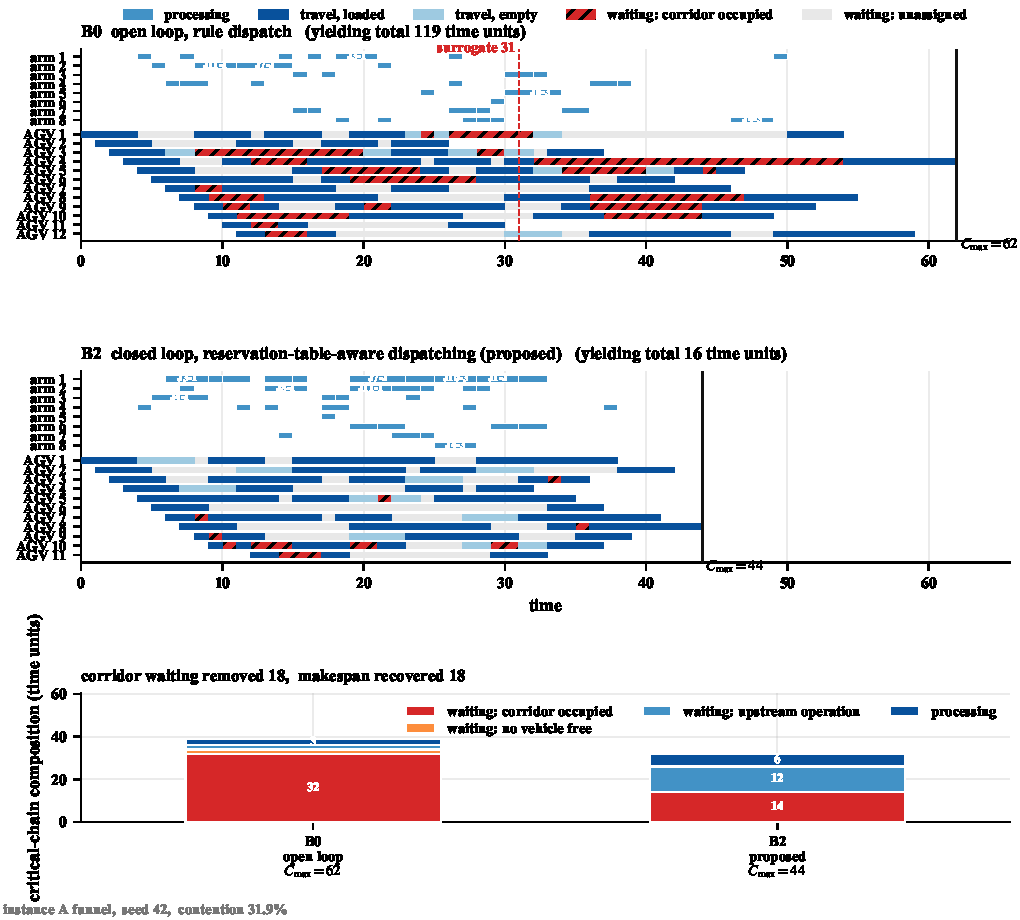
\includegraphics[width=\textwidth]{fig/fig_case.pdf}
\Description{Gantt charts of the open-loop and closed-loop solutions on one
funnel instance, followed by stacked bars decomposing each critical chain by
attribution label.}
\caption{B0 and B2 on one funnel instance.
Top: arms and vehicles on a shared time axis, with empty and loaded legs; a gap between the two legs of one transport is a yielding wait at a berth, a gap between tasks is idle time.
Bottom: critical-chain composition by the labels of Table~\ref{tab:attrib}, with corridor wait removed and makespan reduced.}
\label{fig:case}
%% From fig/fig_case.py and case_study/*.json (ladder_diag.py --case-study).
%% Merges the former fig_case_gantt / fig_case_chain pair.
\end{figure*}

\subsection{Degenerate comparison on public benchmarks}
\label{sec:external}

Comparisons between configurations of one implementation cannot calibrate its absolute level. Without the exclusivity constraint, Eq.~\eqref{eq:excl}, and with $\delta_{\mathrm{ret}}=0$ (Table~\ref{tab:notation}), our model is exactly FJSP\_PT (Section~\ref{sec:Chapter_III}), the \emph{same mathematical problem} as the public benchmarks; neither mechanism is then active, so this anchors the upper-level search, not the framework. We use the \PubNInst{} instances of Homayouni and Fontes~\cite{homayouni2021production} (from Fattahi et al.~\cite{fattahi2007mathematical}) with two vehicles as in Lim and Moon~\cite{lim2023twophase}, and their published travel matrices as $t^{*}$, since \PubNLayoutBad{} are not a shortest-path closure (Section~\ref{sec:instances}); lacking a road network, they admit only this degenerate setting. References are MILP optima for \PubNOpt{} instances~\cite{homayouni2021production} and best published values for $4$~\cite{lim2023twophase}.

All $200$ runs pass validation and never fall below the composite lower bound or a proven optimum. On $\PubNMatch{}/\PubNInst{}$ instances, including all $10$ small ones, the best solution equals the reference digit for digit (Table~\ref{tab:external}); the mean gap is \PubGapMean{}, rising to \PubGapBig{} on the four largest. This reflects search capability, not budget: \PubBudgetRatio{} times the wall-clock time lowers the mean gap of the $10$ \textsc{mfjst} instances only from \PubGapLoBudget{} to \PubGapHiBudget{}, and all runs end by early stopping. On the proven-optimum instances the bound lies a median \PubLBSlack{} below the optimum while the search is at most $\PubLBResidMax$ percentage points above it, so without contention the bound gap is almost entirely bound slack. Since contention can only raise the optimum, the median bound gap of \LBGapMed{} on the self-generated instances \emph{cannot} be read as a search gap.

\begin{table}[t]
\caption{Degenerate comparison on public benchmarks (exclusivity removed). \textsc{opt}: MILP-proven optimum; \textsc{bk}: best published value; gap from the best of \NSeeds{} seeds; asterisk: identical to the reference.}
\label{tab:external}
\centering
\small
%% 由 tab/gen_tables_ladder.py 生成,请勿手工编辑
%% 数据源:clbs/experiments_database/gap_ideal.csv;工序数取自 clbs/database/json/hf/*.json
\begin{tabular}{lrrrrrr}
\toprule
& & & \multicolumn{3}{c}{$C_{\max}$ (time units)} & \\
\cmidrule(lr){4-6}
Instance & Ops & Ref. & \multicolumn{1}{c}{Value} & Best & Mean & Gap \\
\midrule
SFJST01 & 4 & \textsc{opt} & 70 & 70\rlap{$^*$} & 70.0 & 0.00\% \\
SFJST02 & 4 & \textsc{opt} & 111 & 111\rlap{$^*$} & 111.0 & 0.00\% \\
SFJST03 & 6 & \textsc{opt} & 223 & 223\rlap{$^*$} & 223.0 & 0.00\% \\
SFJST04 & 6 & \textsc{opt} & 359 & 359\rlap{$^*$} & 359.0 & 0.00\% \\
SFJST05 & 6 & \textsc{opt} & 123 & 123\rlap{$^*$} & 123.0 & 0.00\% \\
SFJST06 & 9 & \textsc{opt} & 324 & 324\rlap{$^*$} & 324.0 & 0.00\% \\
SFJST07 & 9 & \textsc{opt} & 409 & 409\rlap{$^*$} & 409.0 & 0.00\% \\
SFJST08 & 9 & \textsc{opt} & 269 & 269\rlap{$^*$} & 269.5 & 0.00\% \\
SFJST09 & 9 & \textsc{opt} & 220 & 220\rlap{$^*$} & 222.0 & 0.00\% \\
SFJST10 & 12 & \textsc{opt} & 531 & 531\rlap{$^*$} & 531.0 & 0.00\% \\
MFJST01 & 15 & \textsc{opt} & 485 & 485\rlap{$^*$} & 485.0 & 0.00\% \\
MFJST02 & 15 & \textsc{opt} & 463 & 476 & 483.4 & 2.81\% \\
MFJST03 & 18 & \textsc{opt} & 482 & 482\rlap{$^*$} & 504.7 & 0.00\% \\
MFJST04 & 21 & \textsc{opt} & 576 & 586 & 623.0 & 1.74\% \\
MFJST05 & 21 & \textsc{opt} & 532 & 561 & 592.8 & 5.45\% \\
MFJST06 & 24 & \textsc{opt} & 652 & 677 & 728.3 & 3.83\% \\
MFJST07 & 32 & \textsc{bk} & 898 & 965 & 1023.3 & 7.46\% \\
MFJST08 & 36 & \textsc{bk} & 900 & 970 & 1027.0 & 7.78\% \\
MFJST09 & 44 & \textsc{bk} & 1098 & 1226 & 1279.2 & 11.66\% \\
MFJST10 & 48 & \textsc{bk} & 1230 & 1389 & 1473.0 & 12.93\% \\
\bottomrule
\end{tabular}

\end{table}
%% tab_external() from gap_ideal.csv; the Ops column is counted from
%% hf/*.json (len(proc_time)), not typed.  The same function prints the \Pub*
%% macros.  Edit the CSV, then re-run the script.



\section{Conclusion}

When transport takes longer than processing and congestion concentrates on a few corridors, assignment and conflict-free AGV routing must be decided together. Our closed-loop bilevel framework feeds routing information into decisions through an evaluation path and a decision path, and measures each under the same wall-clock budget.

\subsection{Findings and contributions}
\label{sec:contributions}

\begin{enumerate}[leftmargin=*,topsep=2pt,itemsep=2pt]
\item \textbf{Instance families with controllable contention intensity.} Varying layout, vehicle-to-arm ratio and flexibility, they show a closed-loop gain that broadly rises with contention, to about two and a half times on the most congested instance, but not monotonically.
\item \textbf{Routing-in-the-loop evaluation.} Every chromosome is decodable and evaluated consistently with the conflict model, without repair (Proposition~\ref{prop:decodable}, Lemma~\ref{lem:label}); the closed loop reduces makespan by $\GainLoopRule$ ($p\PLoopRule$) under rule-based and by $\GainLoopProbe$ ($p\PLoopProbe$) under reservation-table-aware dispatching.
\item \textbf{Reservation-table-aware dispatching with output-preserving speed-ups.} A trial query of both legs reduces makespan by a further $\GainProbeLoop$ ($p\PProbeLoop$); pruning and winner-path reuse change neither vehicle nor timetable (Proposition~\ref{prop:speedup_equiv}) and lower the cost multiple from \CostMultBefore{}, at which the gain is lost, to \CostMultAfter{}.
\item \textbf{The two paths differ in magnitude and are not substitutes.} The closed loop is significant after Holm correction on \CellsSigLoopAdj{} of the $\NCases$ instances, dispatching only when pooled ($\GainProbeOpen$, $p\PProbeOpen$, open loop; interval \CIProbeLoop{}, closed loop). The end-to-end gain $\GainEndToEnd$ is slightly below the independent-composition prediction $\GainIndepProduct$, and scheduling before resolving conflicts forgoes the $\GainLoopRule$ of closed-loop evaluation.
\end{enumerate}

\subsection{Limitations and future work}
\label{sec:limitations}
\label{sec:future_work}

\textbf{(1) Instance scope.}
Size and $H=0.3$ are fixed (Section~\ref{sec:features}), so we claim nothing about size, and ``the gain does not rise with $H$'' holds only for the smaller batch of Section~\ref{sec:whichcongestion}; only the three spine instances vary capacity alone, since the grids also change topology and distance (farthest leg \LegDumbbell{} versus \LegGrid{}), and contention intensity does not separate the yielding that reassignment can bypass. The instances are self-generated because no public benchmark has an explicit road network. Future work should remeasure on larger corridor networks, treating bypassability by reassignment and a single dominant bottleneck as separate factors under a new, validated measure.

\textbf{(2) Stability of the dispatching gain.}
Its effect of a few percentage points is of the order of the dispersion across seeds: $\CellsSigProbe$ of $\NCases$ instances are significant before correction and $\CellsSigProbeAdj$ after, so it is confirmed positive only over the $\NPairs$ pooled pairs (interval \CIProbeLoop{}). About ten times more seeds and denser vehicle-to-arm levels would locate where it is stable and test the fleet-size bound of the cost law.

\textbf{(3) Distance from the optimum under contention.}
Search strength is common to all configurations, so their differences are unaffected; without contention, the four largest instances average \PubGapBig{}, gaining only $\PubBudgetGainPP$ percentage points from \PubBudgetRatio{} times the computation, with a seed-to-seed standard deviation of up to \PubCvBig{} of the mean, so the encoding or neighbourhood needs improvement. With contention no optimum is known, and an effect such as \GainProbeLoop{} may be of the order of the distance to it; exact solutions by logic-based Benders decomposition~\cite{vanos2026exact} on small contended instances would separate bound slack from insufficient search and retest the two negative controls under a stronger search.

\textbf{(4) Relative cost of the negative controls.}
The surcharge and yield-record-guided local search were measured as a trade-off between cost per evaluation and number of evaluations: a uniform speed-up keeps the sign, but cutting the cost of one interface alone could change it, as for dispatching. Since the decoder state advances in one direction, re-solving only the part after a perturbation would lower the cost of local search, which should then be remeasured.

\textbf{(5) Static setting.}
Assumption A7 excludes robotic-arm and vehicle failures and dynamic job arrivals, so the results hold for a known job set and failure-free equipment. Under such disruptions, studied for the dynamic flexible job shop~\cite{gui2023dynamic,xiong2024dynamic,dauzereperes2024fjsp}, a mechanism is also valued by how fast it repairs a schedule, which we do not measure, and whether re-solving or local repair is preferable cannot be inferred from the static setting.


%\section*{Acknowledgments}
%This work was supported partly by Key Laboratory of Computer Network and Information Integration (Southeast University) of Ministry of Education of China under Grants NO. 93K-9 and Jiangsu Provincial Key Laboratory of Network and Information Security under Grants No.BM2003201.

%%
%% The next two lines define the bibliography style to be used, and
%% the bibliography file.
\bibliographystyle{ACM-Reference-Format}
\bibliography{reference-base}


%% No appendix.  An empty \appendix leaves a blank TOC/header entry in acmart.

\end{document}
\endinput
%%
